\documentclass[tikz,border=3mm]{standalone}
\usepackage[utf8]{inputenc}
\usepackage[T1]{fontenc}
\usepackage{amsmath,amssymb}
\usepackage{tikz}
\usetikzlibrary{arrows.meta,calc}

\begin{document}
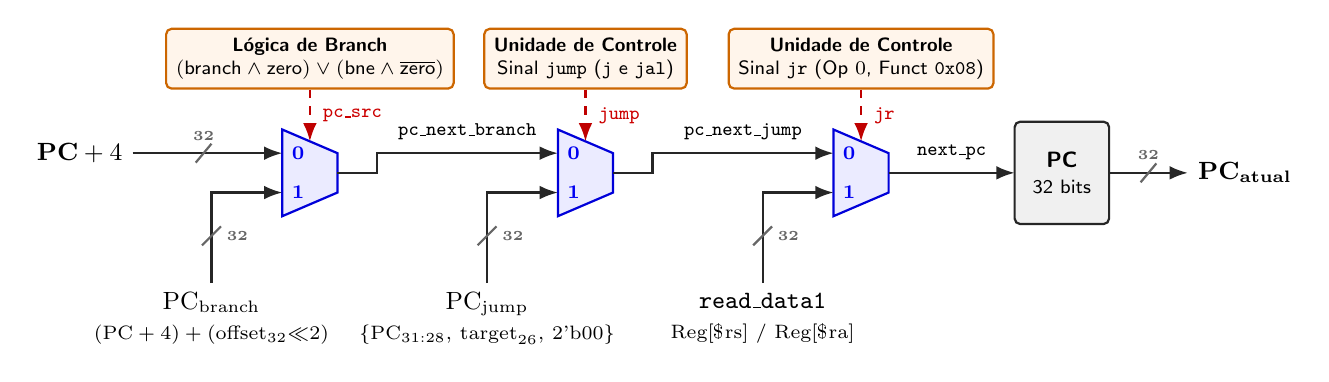
\begin{tikzpicture}[
    >=Latex,
    font=\sffamily\footnotesize,
    muxstyle/.style={draw=blue!85!black, fill=blue!8, thick},
    pcstyle/.style={draw=black!85, fill=gray!12, thick, rounded corners=2pt},
    boxctrl/.style={draw=orange!80!black, fill=orange!8, thick, rounded corners=2pt, font=\sffamily\scriptsize, align=center, inner sep=3.5pt},
    bus/.style={->, thick, draw=black!85},
    ctrl/.style={->, dashed, thick, draw=red!75!black}
]

    % =========================================================================
    % DEFINIÇÃO DOS MULTIPLEXADORES (Trapézios Isósceles Perfeitamente Simétricos)
    % Centro de cada MUX: y = 0
    % Borda esquerda: x, de +0.55 a -0.55 (altura = 1.10)
    % Borda direita:  x + 0.70, de +0.25 a -0.25 (altura = 0.50)
    % Entrada 0: (x, +0.25)
    % Entrada 1: (x, -0.25)
    % Saída:     (x + 0.70, 0)
    % Sel:       (x + 0.35, 0.40)
    % =========================================================================

    % --- MUX 1: Branch (x = 2.4) ---
    \draw[muxstyle] (2.4, 0.55) -- (3.1, 0.25) -- (3.1, -0.25) -- (2.4, -0.55) -- cycle;
    \node[font=\scriptsize\bfseries, text=blue!95!black] at (2.6, 0.25) {0};
    \node[font=\scriptsize\bfseries, text=blue!95!black] at (2.6, -0.25) {1};
    \coordinate (m1_in0) at (2.4, 0.25);
    \coordinate (m1_in1) at (2.4, -0.25);
    \coordinate (m1_out) at (3.1, 0);
    \coordinate (m1_sel) at (2.75, 0.40);

    % --- MUX 2: Jump (x = 5.9) ---
    \draw[muxstyle] (5.9, 0.55) -- (6.6, 0.25) -- (6.6, -0.25) -- (5.9, -0.55) -- cycle;
    \node[font=\scriptsize\bfseries, text=blue!95!black] at (6.1, 0.25) {0};
    \node[font=\scriptsize\bfseries, text=blue!95!black] at (6.1, -0.25) {1};
    \coordinate (m2_in0) at (5.9, 0.25);
    \coordinate (m2_in1) at (5.9, -0.25);
    \coordinate (m2_out) at (6.6, 0);
    \coordinate (m2_sel) at (6.25, 0.40);

    % --- MUX 3: JR (x = 9.4) ---
    \draw[muxstyle] (9.4, 0.55) -- (10.1, 0.25) -- (10.1, -0.25) -- (9.4, -0.55) -- cycle;
    \node[font=\scriptsize\bfseries, text=blue!95!black] at (9.6, 0.25) {0};
    \node[font=\scriptsize\bfseries, text=blue!95!black] at (9.6, -0.25) {1};
    \coordinate (m3_in0) at (9.4, 0.25);
    \coordinate (m3_in1) at (9.4, -0.25);
    \coordinate (m3_out) at (10.1, 0);
    \coordinate (m3_sel) at (9.75, 0.40);

    % --- Registrador PC (x = 11.7) ---
    \draw[pcstyle] (11.7, -0.65) rectangle (12.9, 0.65);
    \node[align=center] at (12.3, 0) {\textbf{PC}\\\scriptsize 32 bits};
    \coordinate (pc_in) at (11.7, 0);
    \coordinate (pc_out) at (12.9, 0);

    % =========================================================================
    % BARRAMENTO PRINCIPAL HORIZONTAL E CONEXÕES DOS MUXES
    % =========================================================================
    % Entrada PC + 4 (em y = 0.25)
    \draw[bus] (0.5, 0.25) -- (m1_in0)
        node[at start, left, font=\small\bfseries] {$\text{PC}+4$};

    % MUX 1 out -> MUX 2 in0 (Degrau suave em x = 3.6)
    \draw[bus] (m1_out) -- (3.6, 0) |- (m2_in0)
        node[pos=0.75, above=1pt, font=\scriptsize\ttfamily] {pc\_next\_branch};

    % MUX 2 out -> MUX 3 in0 (Degrau suave em x = 7.1)
    \draw[bus] (m2_out) -- (7.1, 0) |- (m3_in0)
        node[pos=0.75, above=1pt, font=\scriptsize\ttfamily] {pc\_next\_jump};

    % MUX 3 out -> PC in (Reta horizontal pura em y = 0!)
    \draw[bus] (m3_out) -- (pc_in)
        node[midway, above=1pt, font=\scriptsize\ttfamily\bfseries] {next\_pc};

    % PC out -> Saída
    \draw[bus] (pc_out) -- ++(1.0, 0)
        node[at end, right, font=\small\bfseries] {$\text{PC}_{\text{atual}}$};

    % Traço / 32 na entrada e na saída
    \draw[thick, black!60] (1.3, 0.13) -- (1.5, 0.37);
    \node[font=\tiny\bfseries, text=black!60] at (1.4, 0.47) {32};

    \draw[thick, black!60] (13.3, -0.12) -- (13.5, 0.12);
    \node[font=\tiny\bfseries, text=black!60] at (13.4, 0.22) {32};

    % =========================================================================
    % ENTRADAS DE SALTO (VINDO DE BAIXO)
    % =========================================================================
    % 1. Branch Target
    \draw[bus] (1.5, -1.4) |- (m1_in1);
    \node[align=center, font=\small] at (1.5, -1.85) {
        $\text{PC}_{\text{branch}}$\\
        \scriptsize$(\text{PC}+4)+(\text{offset}_{32}{\ll}2)$
    };
    \draw[thick, black!60] (1.38, -0.92) -- (1.62, -0.68);
    \node[font=\tiny\bfseries, text=black!60, right=2pt] at (1.5, -0.80) {32};

    % 2. Jump Target
    \draw[bus] (5.0, -1.4) |- (m2_in1);
    \node[align=center, font=\small] at (5.0, -1.85) {
        $\text{PC}_{\text{jump}}$\\
        \scriptsize$\{\text{PC}_{31:28},\,\text{target}_{26},\,\text{2'b00}\}$
    };
    \draw[thick, black!60] (4.88, -0.92) -- (5.12, -0.68);
    \node[font=\tiny\bfseries, text=black!60, right=2pt] at (5.0, -0.80) {32};

    % 3. JR Register Target
    \draw[bus] (8.5, -1.4) |- (m3_in1);
    \node[align=center, font=\small] at (8.5, -1.85) {
        \texttt{read\_data1}\\
        \scriptsize Reg[\$rs] / Reg[\$ra]
    };
    \draw[thick, black!60] (8.38, -0.92) -- (8.62, -0.68);
    \node[font=\tiny\bfseries, text=black!60, right=2pt] at (8.5, -0.80) {32};

    % =========================================================================
    % SINAIS DE CONTROLE (VINDO DO TOPO)
    % =========================================================================
    % 1. Lógica pc_src
    \node[boxctrl] (ctrl1) at (2.75, 1.45) {
        \textbf{Lógica de Branch}\\
        $(\text{branch} \land \text{zero}) \lor (\text{bne} \land \overline{\text{zero}})$
    };
    \draw[ctrl] (ctrl1.south) -- (m1_sel)
        node[midway, right=1pt, font=\scriptsize\ttfamily\bfseries, text=red!80!black] {pc\_src};

    % 2. Decodificador jump
    \node[boxctrl] (ctrl2) at (6.25, 1.45) {
        \textbf{Unidade de Controle}\\
        Sinal \texttt{jump} (\texttt{j} e \texttt{jal})
    };
    \draw[ctrl] (ctrl2.south) -- (m2_sel)
        node[midway, right=1pt, font=\scriptsize\ttfamily\bfseries, text=red!80!black] {jump};

    % 3. Decodificador jr
    \node[boxctrl] (ctrl3) at (9.75, 1.45) {
        \textbf{Unidade de Controle}\\
        Sinal \texttt{jr} (Op $0$, Funct \texttt{0x08})
    };
    \draw[ctrl] (ctrl3.south) -- (m3_sel)
        node[midway, right=1pt, font=\scriptsize\ttfamily\bfseries, text=red!80!black] {jr};

\end{tikzpicture}
\end{document}
